% !TEX root = ../main.tex

\begin{frame}{New Voctomix Features}
	\begin{itemize}
		\item Voctomix has presets now!
		\begin{itemize}
			\item Lecture mode with slides and camera on one button!
			\item No more accidents with the slides in small picture
		\end{itemize}
		\item Use lecture mode more often
	\end{itemize}
\end{frame}

\begin{frame}{New Voctomix Features}
	\begin{figure}
		\centering
		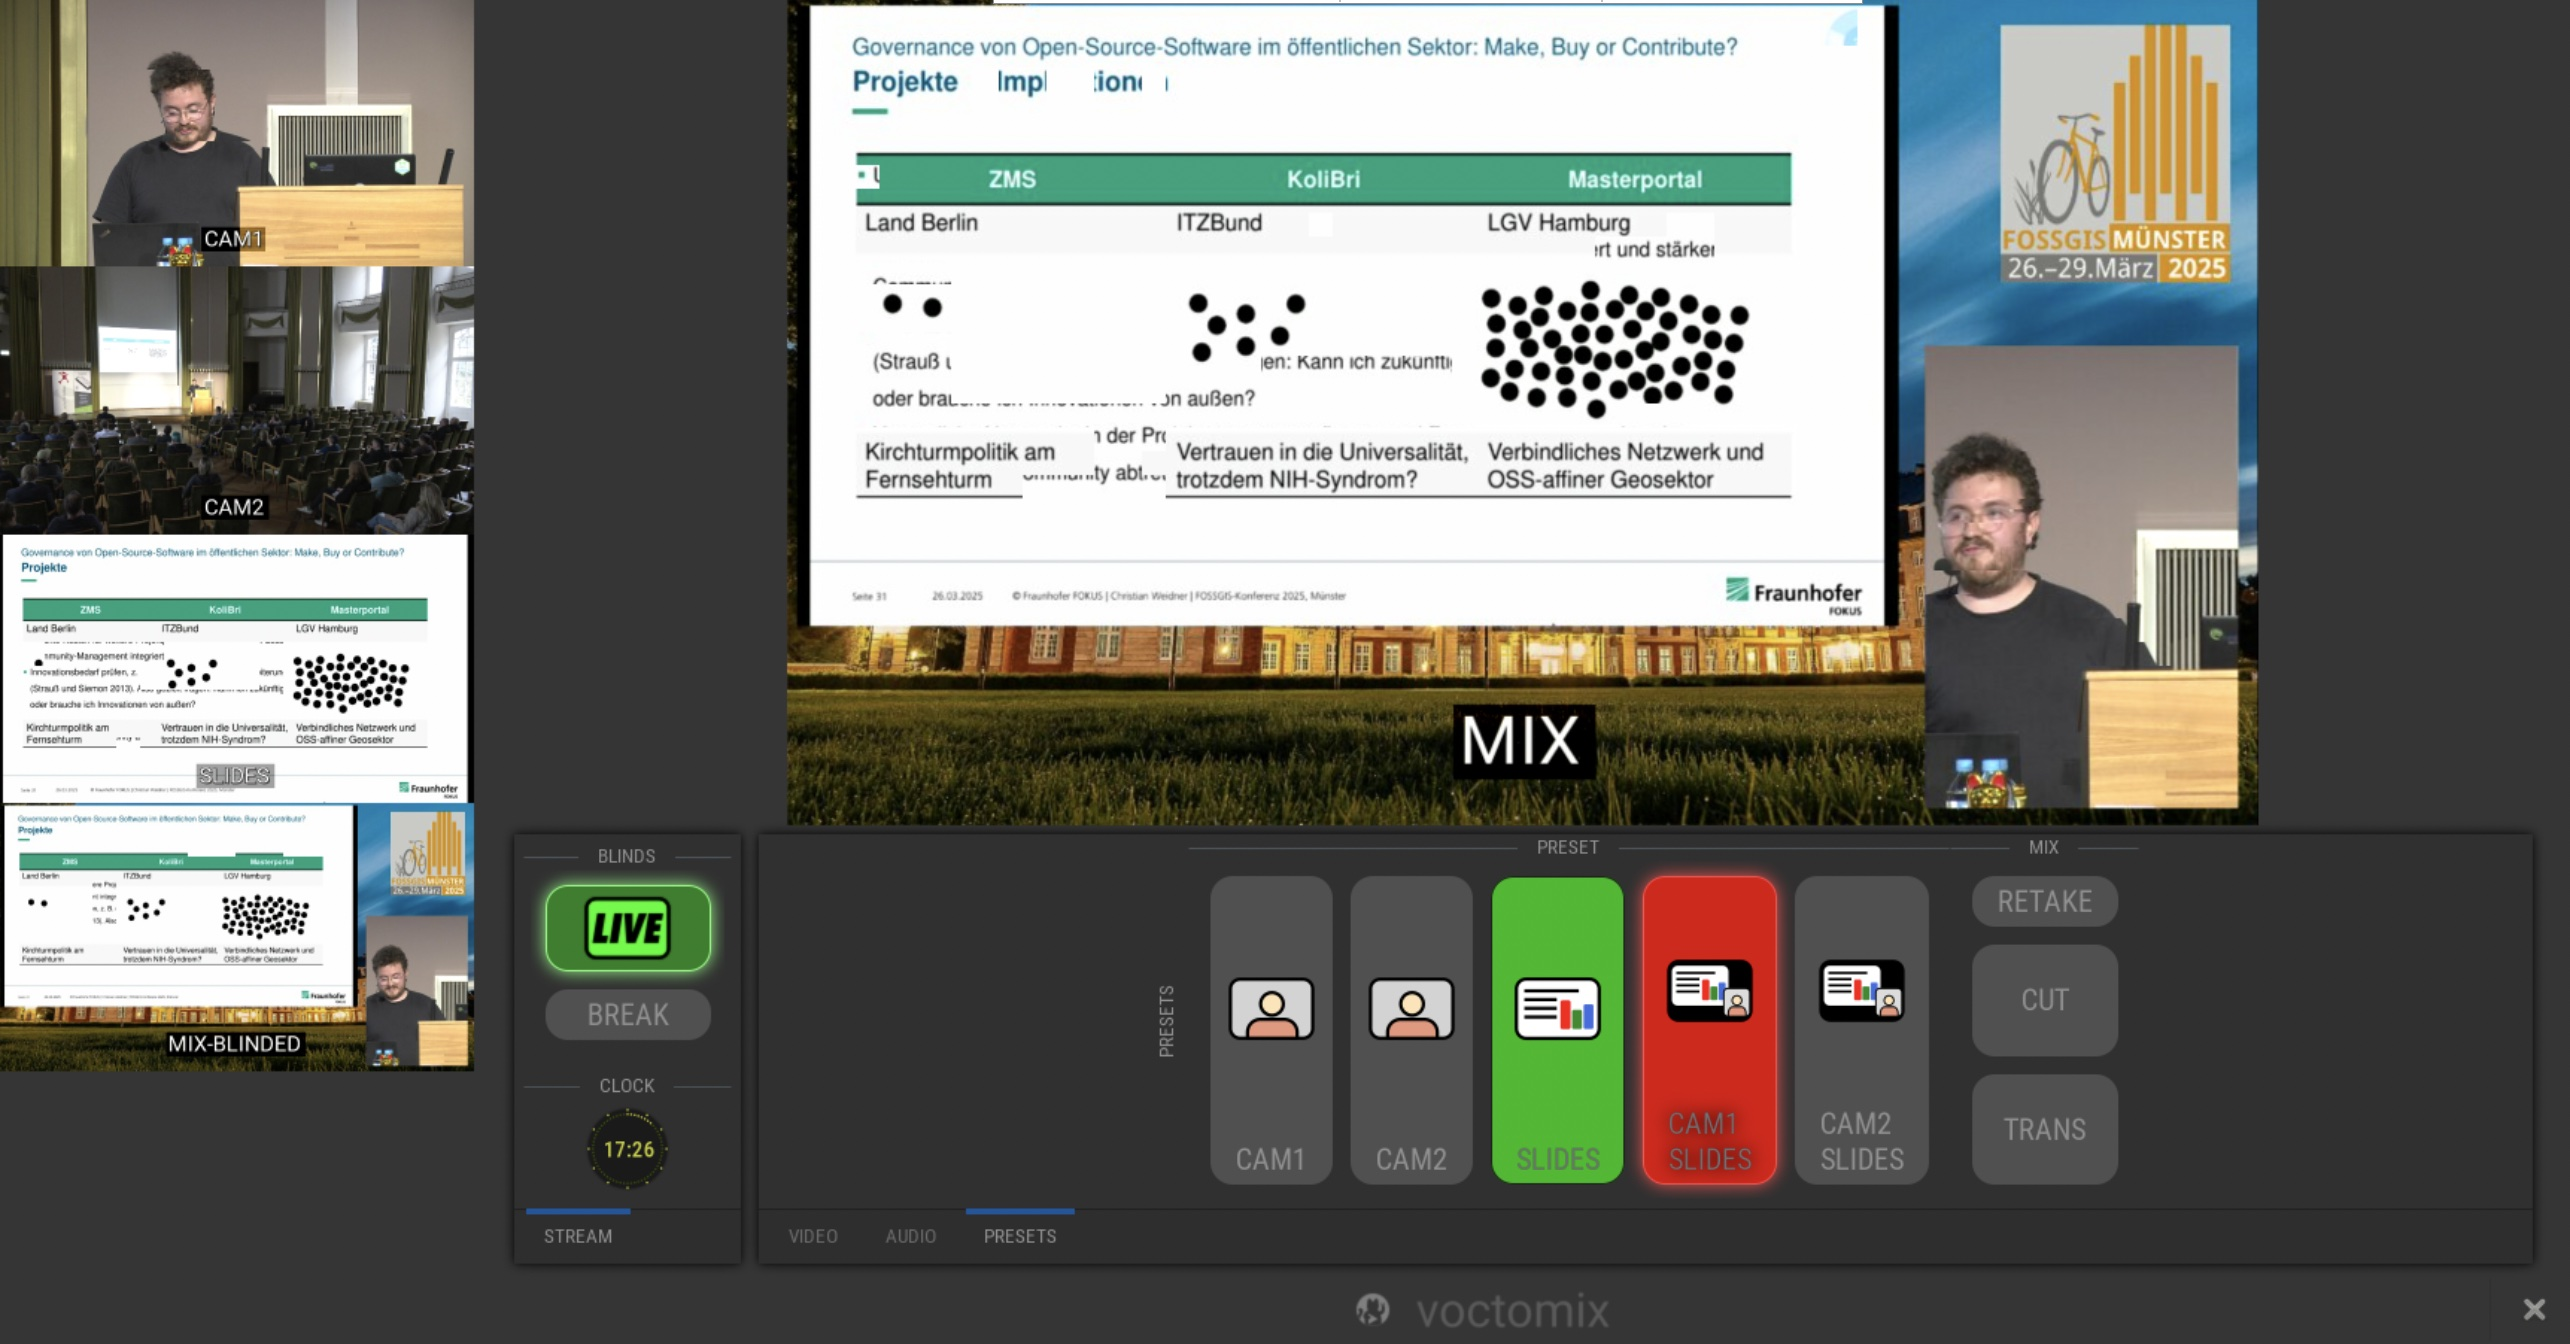
\includegraphics[width=0.9\textwidth]{images/voctomix2-presets-lecture.jpg}
		\caption{Voctomix2 Presets: Lecture Mode}
	\end{figure}
\end{frame}

\begin{frame}{New Voctomix Features}
	\begin{figure}
		\centering
		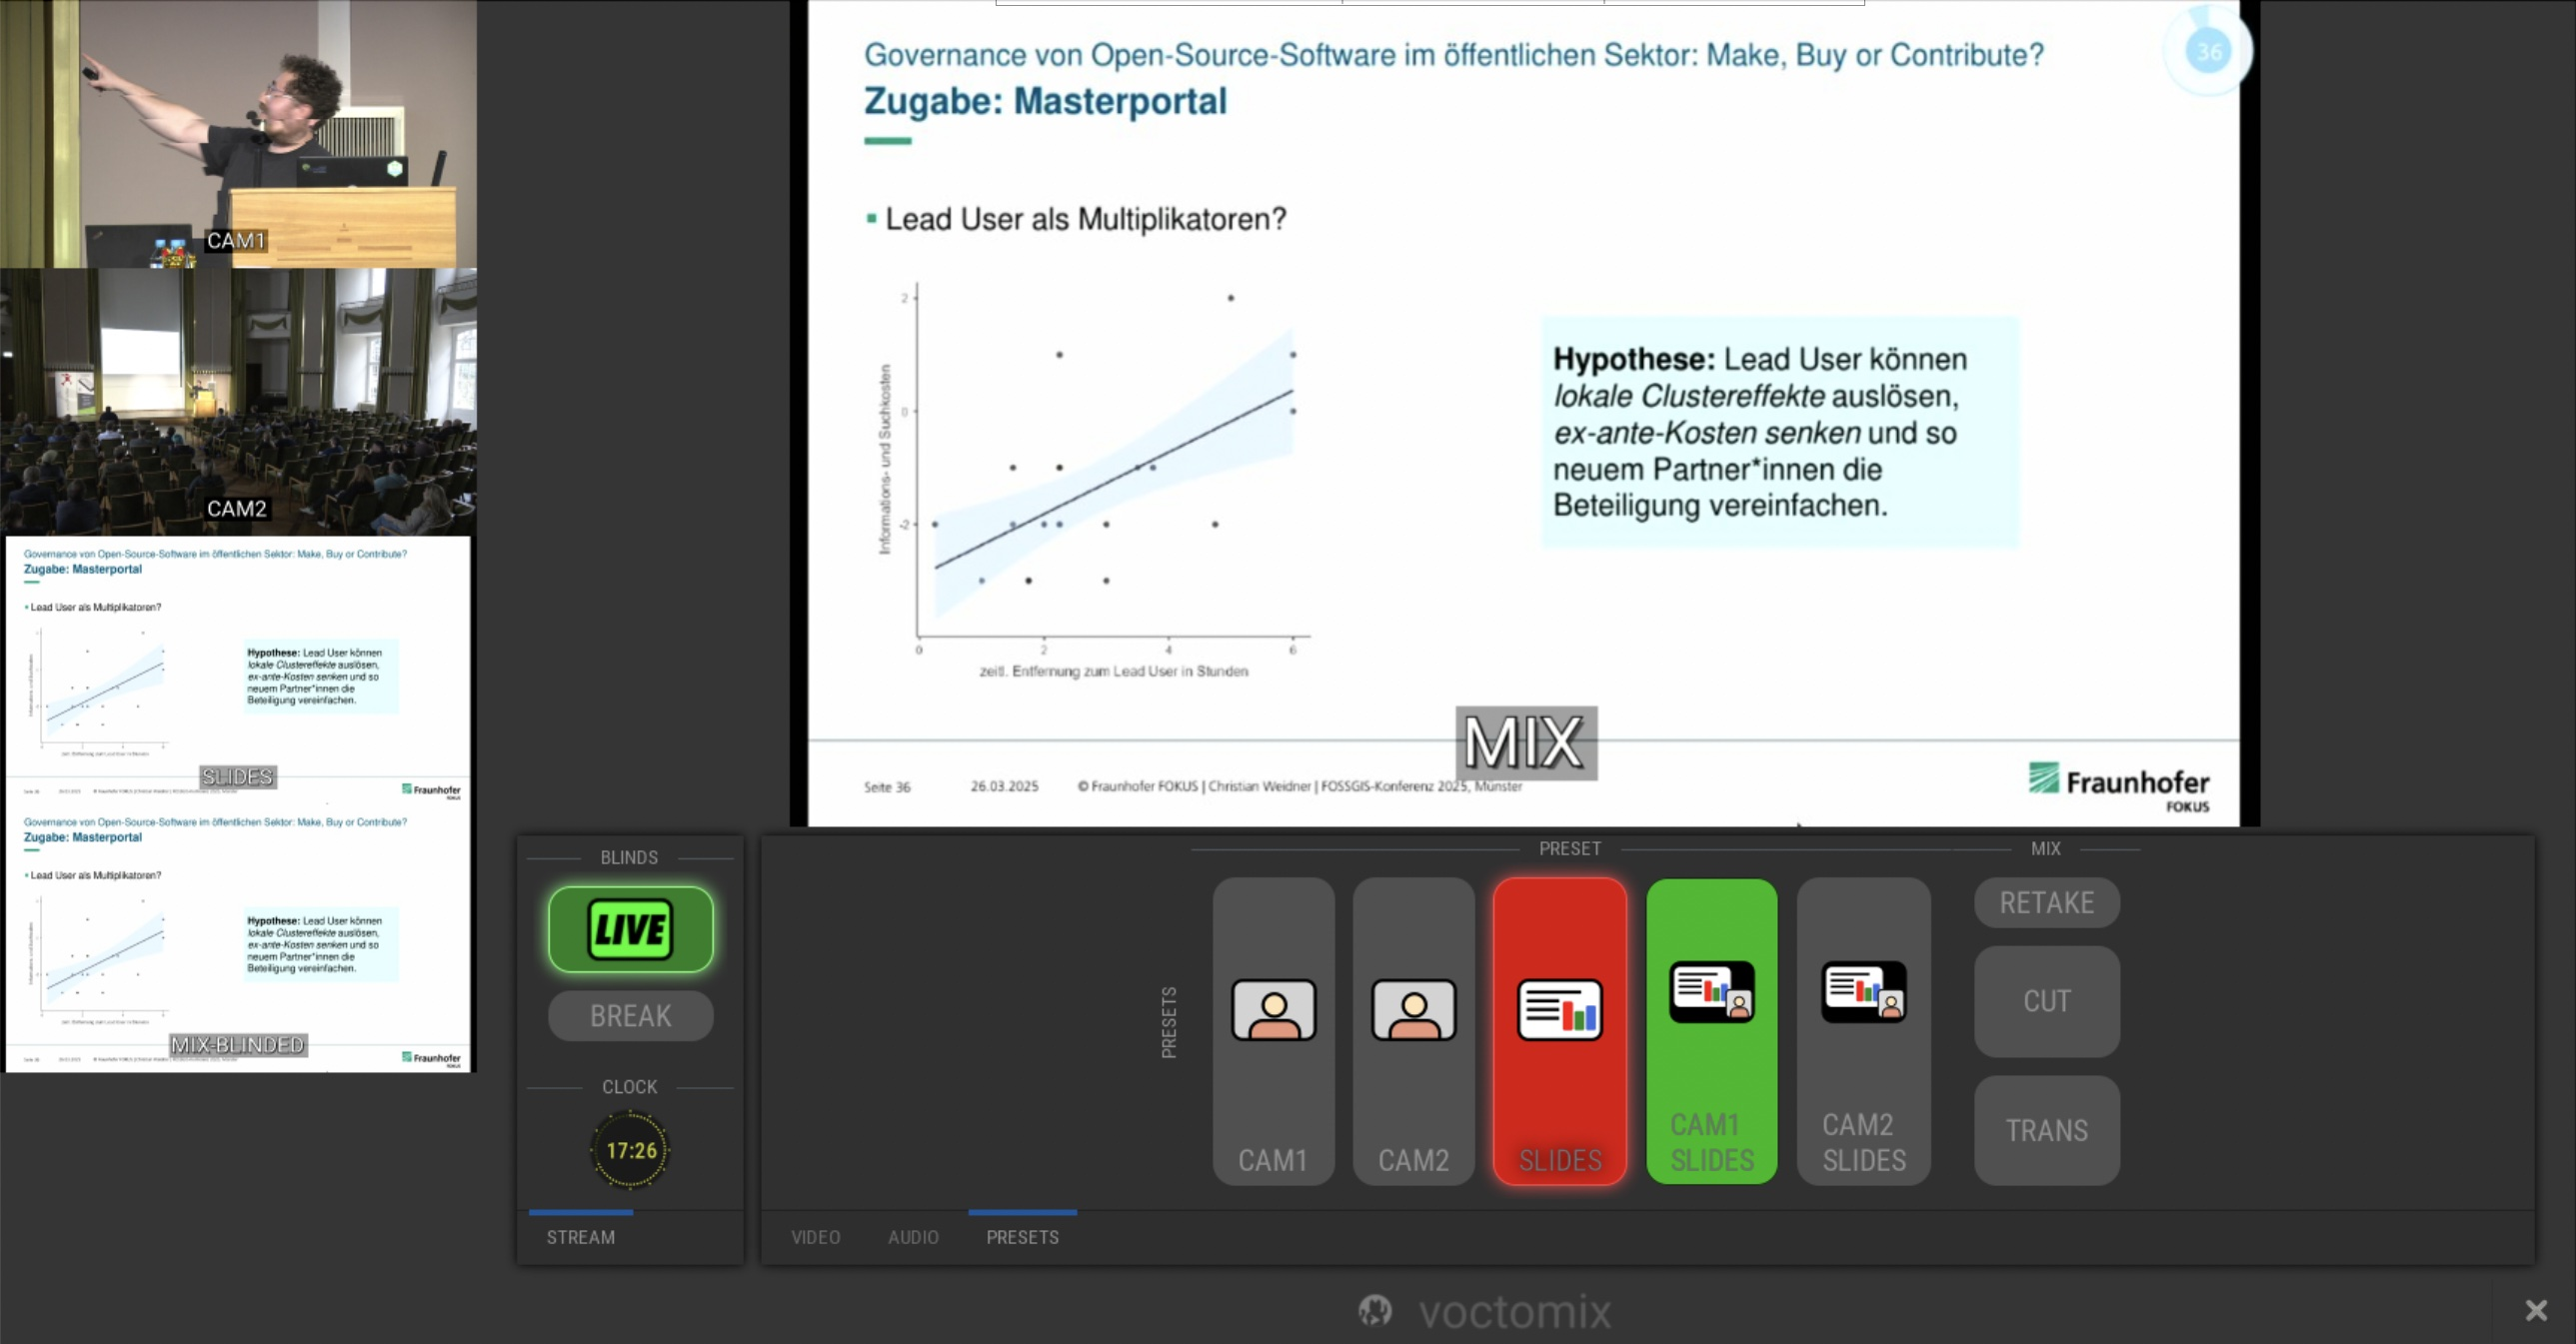
\includegraphics[width=0.9\textwidth]{images/voctomix2-presets-slides.jpg}
		\caption{Voctomix2 Presets: Slides Fullscreen}
	\end{figure}
\end{frame}
